\section{Simulation Analysis}
\label{sec:simulation}

In this section, Ngspice was used in order to simulate the Bandpass Filter. A brief description of the circuit modeled in NGspice is going to be presented and a comparison between the values obtained in NGspice and the ones in Octave is going to be done as well. In order to do that, OP AMP of the given models were used and the rest of the components specifications changed to be on par with the values through MatLab.

In the next sections we are interested in ... . The measurement of these parameters and the overall performance of the circuit is well represented in the section \ref{merit}.\par 

%Results
\begin{table}[H] \centering
\begin{tabular}{|
>{\columncolor[HTML]{FFCC67}}l |c|}
\hline
\multicolumn{2}{|l|}{\cellcolor[HTML]{EABD8B}Name - Value} \\ \hline
V-Gain & 34.1988\\ \hline
Bandwidth & 1.22501E+06\\ \hline
CO-lowerFreq & 15.8734\\ \hline
CO-higherFreq & 1.22503E+06\\ \hline

\end{tabular}
\caption{Results}
\end{table}

%Zin
\begin{table}[H] \centering
\begin{tabular}{|
>{\columncolor[HTML]{FFCC67}}l |c|}
\hline
\multicolumn{2}{|l|}{\cellcolor[HTML]{EABD8B}Name - Value} \\ \hline
Zin & 999.002 + -7.3282 j\\ \hline

\end{tabular}
\caption{Zin}
\end{table}


%Gain comparison

\begin{figure}[H] 
\centering
\begin{subfigure}{0.3\textwidth}
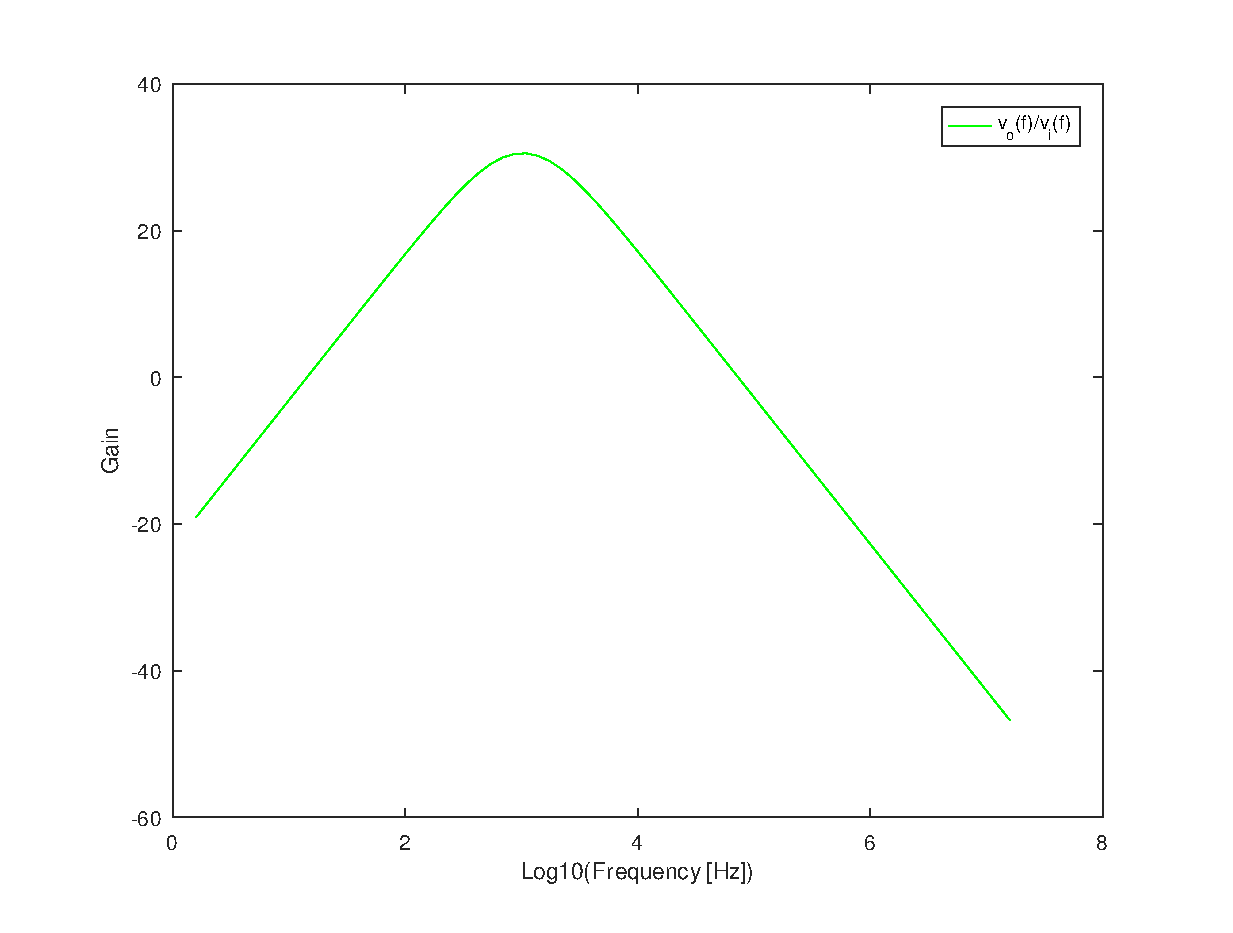
\includegraphics[width=\textwidth]{theo.eps}
\caption{OCTAVE}
\label{Octave_gain}
\end{subfigure}
\begin{subfigure}{0.3\textwidth}
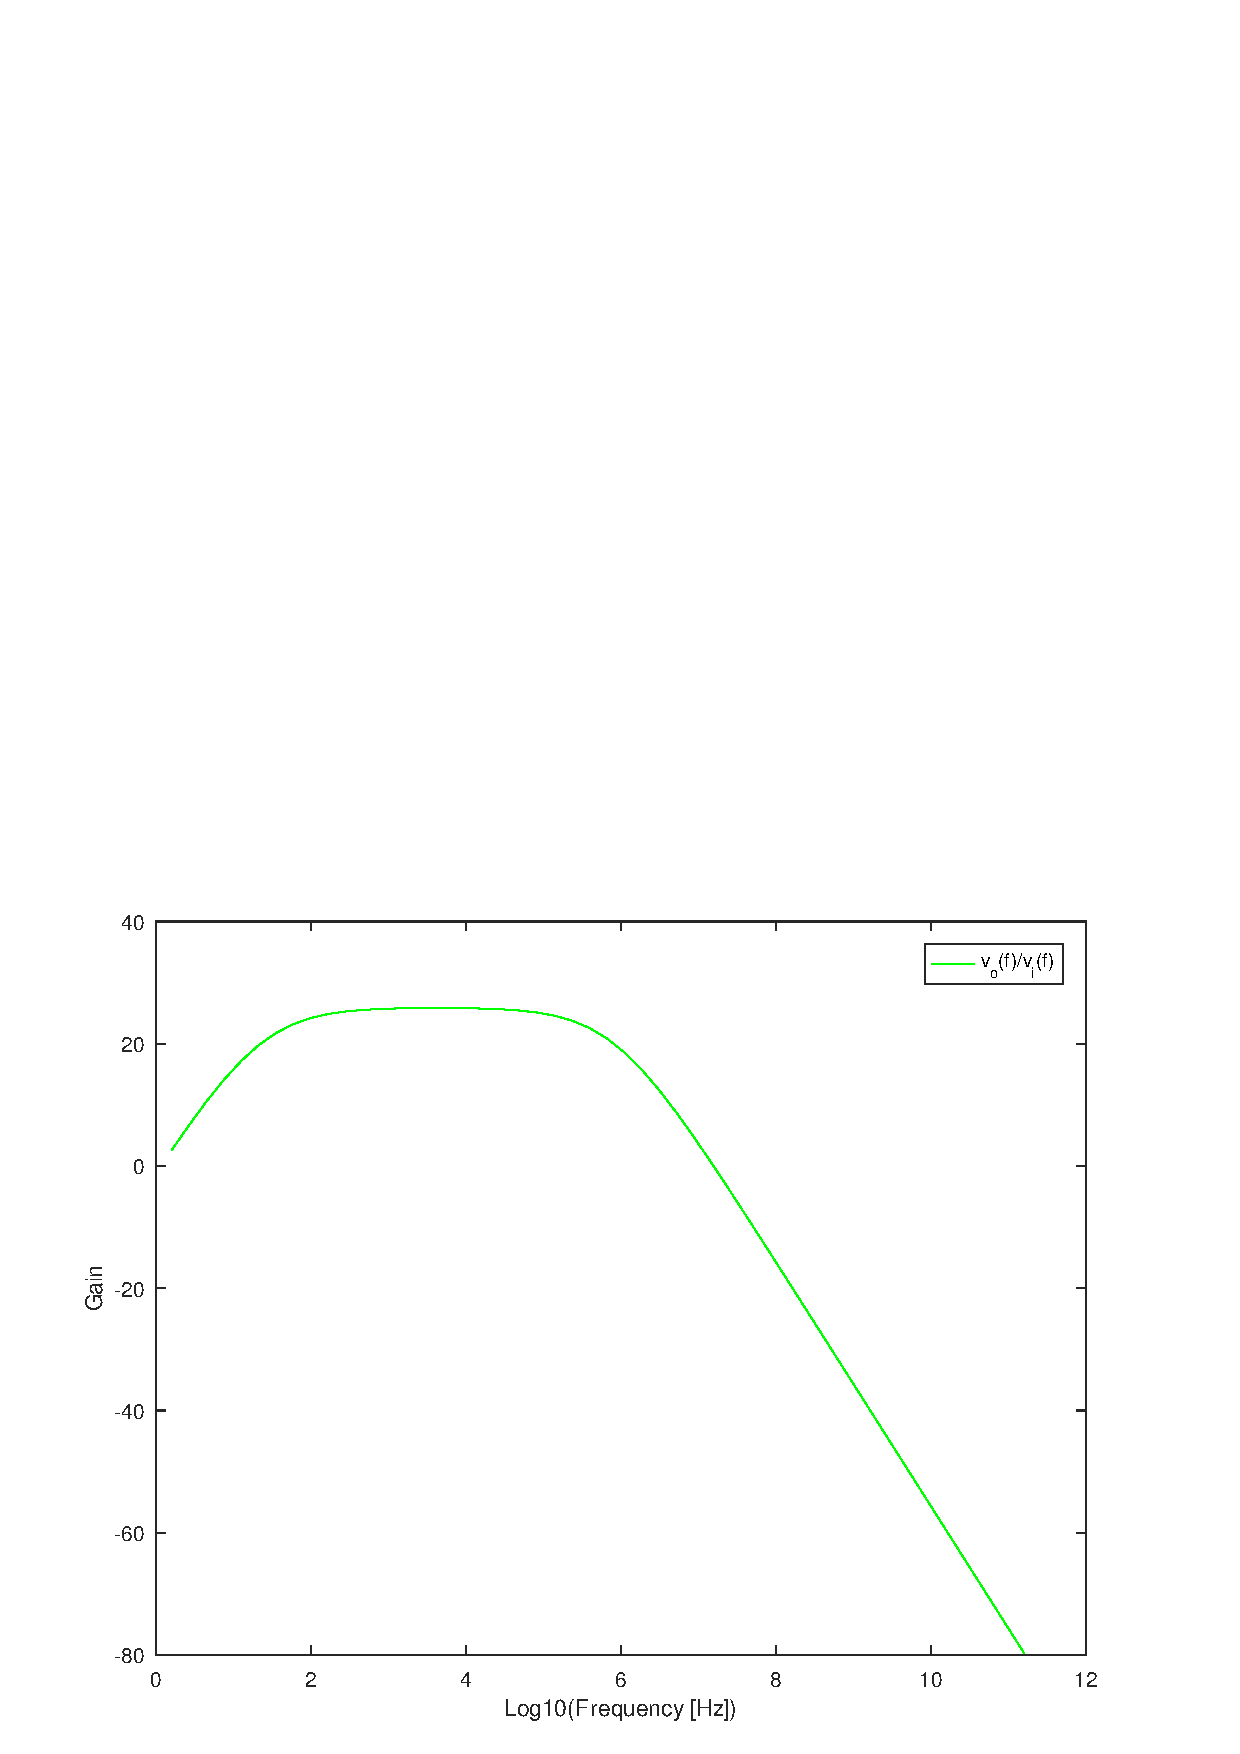
\includegraphics[width=\textwidth]{Gain.pdf}
\caption{NGSPICE}
\label{Ngspice_gain}
\end{subfigure}
\caption{Gain}
\end{figure}

%vo1f

%\begin{figure}[H] 
%\centering
%\begin{subfigure}{0.3\textwidth}
%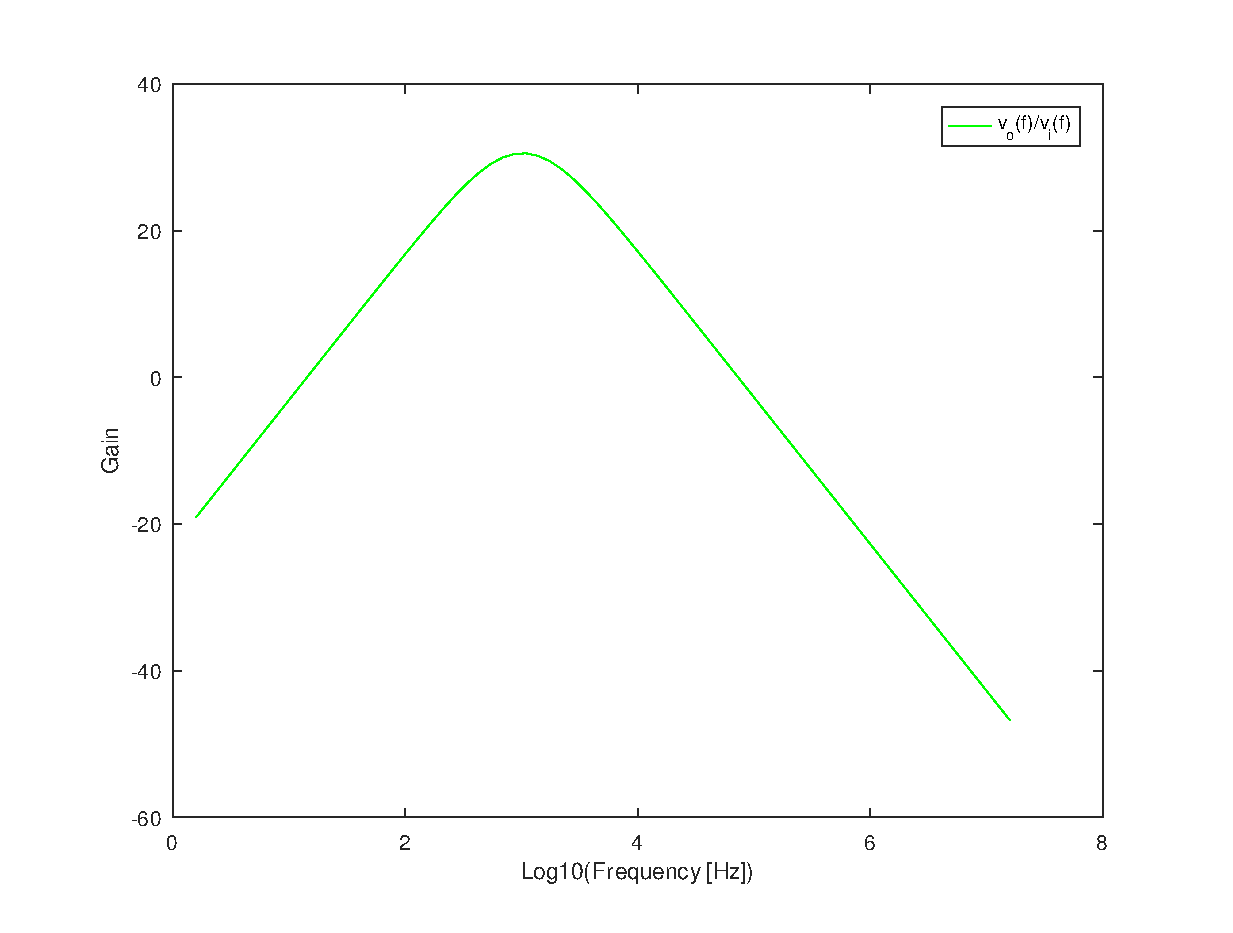
\includegraphics[width=\textwidth]{theo.eps}
%\caption{OCTAVE}
%\label{Octave_vo1f}
%\end{subfigure}
%\begin{subfigure}{0.3\textwidth}
%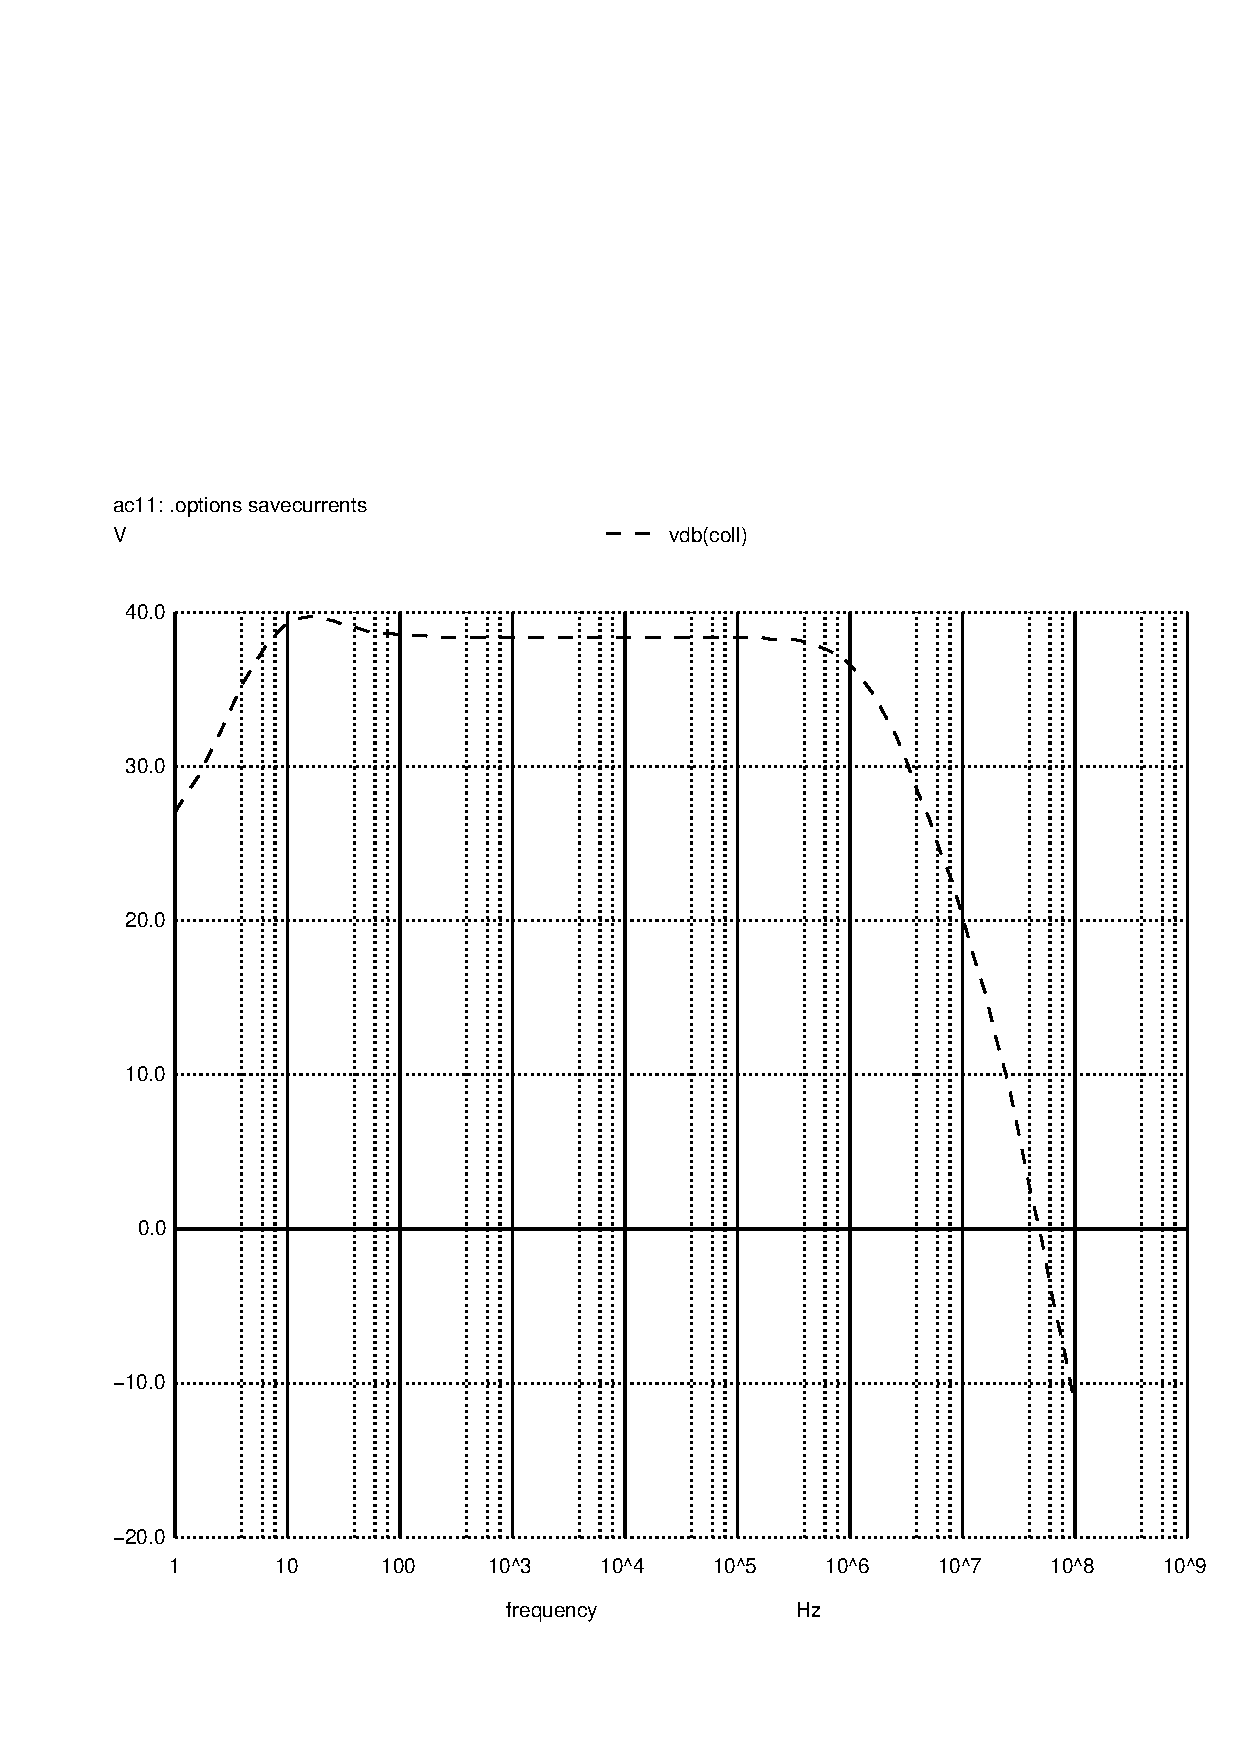
\includegraphics[width=\textwidth]{vo1f.pdf}
%\caption{NGSPICE}
%\label{Ngspice_vo1f}
%\end{subfigure}
%\caption{vo1f}
%\end{figure}



\subsection{Merit Results}
\label{merit}

From the results obtained through the Ngspice simulation and considering we used the data shown in table 1, we can compute the merit using the formula given in the lab assignment, represented in the Introduction.

The values of cost and merit are represented in the next table:

\begin{table}[H] \centering
\begin{tabular}{|
>{\columncolor[HTML]{FFCC67}}l |c|}
\hline
\multicolumn{2}{|l|}{\cellcolor[HTML]{EABD8B}Name - Value} \\ \hline
Cost & 2619.6\\ \hline
merit & 1262.83\\ \hline

\end{tabular}
\caption{Cost and Merit}
\end{table}

To obtain the best values for the circuit, we've used the matlab simulink to optimize them for the best merit.
